% Created by tikzDevice version 0.12
% !TEX encoding = UTF-8 Unicode
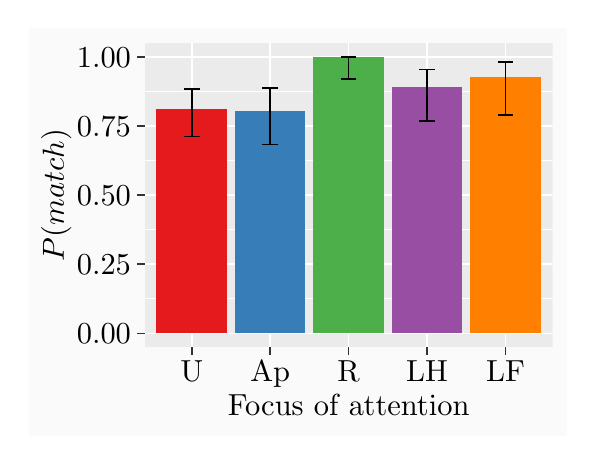
\begin{tikzpicture}[x=1pt,y=1pt]
\definecolor{fillColor}{RGB}{255,255,255}
\path[use as bounding box,fill=fillColor,fill opacity=0.00] (0,0) rectangle (195.19,147.70);
\begin{scope}
\path[clip] (  0.00,  0.00) rectangle (195.19,147.70);
\definecolor{drawColor}{RGB}{255,255,255}
\definecolor{fillColor}{gray}{0.98}

\path[draw=drawColor,line width= 0.6pt,line join=round,line cap=round,fill=fillColor] (  0.00, -0.00) rectangle (195.19,147.70);
\end{scope}
\begin{scope}
\path[clip] ( 42.27, 32.24) rectangle (189.69,142.20);
\definecolor{fillColor}{gray}{0.92}

\path[fill=fillColor] ( 42.27, 32.24) rectangle (189.69,142.20);
\definecolor{drawColor}{RGB}{255,255,255}

\path[draw=drawColor,line width= 0.3pt,line join=round] ( 42.27, 49.73) --
	(189.69, 49.73);

\path[draw=drawColor,line width= 0.3pt,line join=round] ( 42.27, 74.73) --
	(189.69, 74.73);

\path[draw=drawColor,line width= 0.3pt,line join=round] ( 42.27, 99.72) --
	(189.69, 99.72);

\path[draw=drawColor,line width= 0.3pt,line join=round] ( 42.27,124.71) --
	(189.69,124.71);

\path[draw=drawColor,line width= 0.6pt,line join=round] ( 42.27, 37.24) --
	(189.69, 37.24);

\path[draw=drawColor,line width= 0.6pt,line join=round] ( 42.27, 62.23) --
	(189.69, 62.23);

\path[draw=drawColor,line width= 0.6pt,line join=round] ( 42.27, 87.22) --
	(189.69, 87.22);

\path[draw=drawColor,line width= 0.6pt,line join=round] ( 42.27,112.21) --
	(189.69,112.21);

\path[draw=drawColor,line width= 0.6pt,line join=round] ( 42.27,137.21) --
	(189.69,137.21);

\path[draw=drawColor,line width= 0.6pt,line join=round] ( 59.28, 32.24) --
	( 59.28,142.20);

\path[draw=drawColor,line width= 0.6pt,line join=round] ( 87.63, 32.24) --
	( 87.63,142.20);

\path[draw=drawColor,line width= 0.6pt,line join=round] (115.98, 32.24) --
	(115.98,142.20);

\path[draw=drawColor,line width= 0.6pt,line join=round] (144.33, 32.24) --
	(144.33,142.20);

\path[draw=drawColor,line width= 0.6pt,line join=round] (172.68, 32.24) --
	(172.68,142.20);
\definecolor{fillColor}{RGB}{228,26,28}

\path[fill=fillColor] ( 46.52, 37.24) rectangle ( 72.04,118.32);
\definecolor{fillColor}{RGB}{55,126,184}

\path[fill=fillColor] ( 74.87, 37.24) rectangle (100.39,117.52);
\definecolor{fillColor}{RGB}{77,175,74}

\path[fill=fillColor] (103.22, 37.24) rectangle (128.74,137.21);
\definecolor{fillColor}{RGB}{152,78,163}

\path[fill=fillColor] (131.57, 37.24) rectangle (157.08,126.10);
\definecolor{fillColor}{RGB}{255,127,0}

\path[fill=fillColor] (159.92, 37.24) rectangle (185.43,129.89);
\definecolor{drawColor}{RGB}{0,0,0}

\path[draw=drawColor,line width= 0.6pt,line join=round] ( 56.45,125.52) --
	( 62.12,125.52);

\path[draw=drawColor,line width= 0.6pt,line join=round] ( 59.28,125.52) --
	( 59.28,108.42);

\path[draw=drawColor,line width= 0.6pt,line join=round] ( 56.45,108.42) --
	( 62.12,108.42);

\path[draw=drawColor,line width= 0.6pt,line join=round] ( 84.79,125.91) --
	( 90.46,125.91);

\path[draw=drawColor,line width= 0.6pt,line join=round] ( 87.63,125.91) --
	( 87.63,105.54);

\path[draw=drawColor,line width= 0.6pt,line join=round] ( 84.79,105.54) --
	( 90.46,105.54);

\path[draw=drawColor,line width= 0.6pt,line join=round] (113.14,137.21) --
	(118.81,137.21);

\path[draw=drawColor,line width= 0.6pt,line join=round] (115.98,137.21) --
	(115.98,129.21);

\path[draw=drawColor,line width= 0.6pt,line join=round] (113.14,129.21) --
	(118.81,129.21);

\path[draw=drawColor,line width= 0.6pt,line join=round] (141.49,132.61) --
	(147.16,132.61);

\path[draw=drawColor,line width= 0.6pt,line join=round] (144.33,132.61) --
	(144.33,113.90);

\path[draw=drawColor,line width= 0.6pt,line join=round] (141.49,113.90) --
	(147.16,113.90);

\path[draw=drawColor,line width= 0.6pt,line join=round] (169.84,135.30) --
	(175.51,135.30);

\path[draw=drawColor,line width= 0.6pt,line join=round] (172.68,135.30) --
	(172.68,116.21);

\path[draw=drawColor,line width= 0.6pt,line join=round] (169.84,116.21) --
	(175.51,116.21);
\end{scope}
\begin{scope}
\path[clip] (  0.00,  0.00) rectangle (195.19,147.70);
\definecolor{drawColor}{RGB}{0,0,0}

\node[text=drawColor,anchor=base east,inner sep=0pt, outer sep=0pt, scale=  1.10] at ( 37.32, 33.45) {0.00};

\node[text=drawColor,anchor=base east,inner sep=0pt, outer sep=0pt, scale=  1.10] at ( 37.32, 58.44) {0.25};

\node[text=drawColor,anchor=base east,inner sep=0pt, outer sep=0pt, scale=  1.10] at ( 37.32, 83.43) {0.50};

\node[text=drawColor,anchor=base east,inner sep=0pt, outer sep=0pt, scale=  1.10] at ( 37.32,108.43) {0.75};

\node[text=drawColor,anchor=base east,inner sep=0pt, outer sep=0pt, scale=  1.10] at ( 37.32,133.42) {1.00};
\end{scope}
\begin{scope}
\path[clip] (  0.00,  0.00) rectangle (195.19,147.70);
\definecolor{drawColor}{gray}{0.20}

\path[draw=drawColor,line width= 0.6pt,line join=round] ( 39.52, 37.24) --
	( 42.27, 37.24);

\path[draw=drawColor,line width= 0.6pt,line join=round] ( 39.52, 62.23) --
	( 42.27, 62.23);

\path[draw=drawColor,line width= 0.6pt,line join=round] ( 39.52, 87.22) --
	( 42.27, 87.22);

\path[draw=drawColor,line width= 0.6pt,line join=round] ( 39.52,112.21) --
	( 42.27,112.21);

\path[draw=drawColor,line width= 0.6pt,line join=round] ( 39.52,137.21) --
	( 42.27,137.21);
\end{scope}
\begin{scope}
\path[clip] (  0.00,  0.00) rectangle (195.19,147.70);
\definecolor{drawColor}{gray}{0.20}

\path[draw=drawColor,line width= 0.6pt,line join=round] ( 59.28, 29.49) --
	( 59.28, 32.24);

\path[draw=drawColor,line width= 0.6pt,line join=round] ( 87.63, 29.49) --
	( 87.63, 32.24);

\path[draw=drawColor,line width= 0.6pt,line join=round] (115.98, 29.49) --
	(115.98, 32.24);

\path[draw=drawColor,line width= 0.6pt,line join=round] (144.33, 29.49) --
	(144.33, 32.24);

\path[draw=drawColor,line width= 0.6pt,line join=round] (172.68, 29.49) --
	(172.68, 32.24);
\end{scope}
\begin{scope}
\path[clip] (  0.00,  0.00) rectangle (195.19,147.70);
\definecolor{drawColor}{RGB}{0,0,0}

\node[text=drawColor,anchor=base,inner sep=0pt, outer sep=0pt, scale=  1.10] at ( 59.28, 19.71) {U};

\node[text=drawColor,anchor=base,inner sep=0pt, outer sep=0pt, scale=  1.10] at ( 87.63, 19.71) {Ap};

\node[text=drawColor,anchor=base,inner sep=0pt, outer sep=0pt, scale=  1.10] at (115.98, 19.71) {R};

\node[text=drawColor,anchor=base,inner sep=0pt, outer sep=0pt, scale=  1.10] at (144.33, 19.71) {LH};

\node[text=drawColor,anchor=base,inner sep=0pt, outer sep=0pt, scale=  1.10] at (172.68, 19.71) {LF};
\end{scope}
\begin{scope}
\path[clip] (  0.00,  0.00) rectangle (195.19,147.70);
\definecolor{drawColor}{RGB}{0,0,0}

\node[text=drawColor,anchor=base,inner sep=0pt, outer sep=0pt, scale=  1.10] at (115.98,  7.44) {Focus of attention};
\end{scope}
\begin{scope}
\path[clip] (  0.00,  0.00) rectangle (195.19,147.70);
\definecolor{drawColor}{RGB}{0,0,0}

\node[text=drawColor,rotate= 90.00,anchor=base,inner sep=0pt, outer sep=0pt, scale=  1.10] at ( 13.08, 87.22) {\(P(match)\)};
\end{scope}
\end{tikzpicture}
